\documentclass[../DD0.tex]{subfiles}

\begin{document}

\section{Architectural Design}
\label{sec:arcdes}

  \subsection{Overview}
  \label{sec:overview}

    The architecture is a three-tier architecture (Figure~\ref{fig:overallarchitecture}): it allows to separate clearly \textit{presentation} layer, \textit{business} layer and \textit{data} layer. These sets of components will communicate through defined interfaces and will be treated as black boxes during their interaction. This modular approach enhances modifiability and extensibility.

    \begin{figure}[h!]
      \centering
      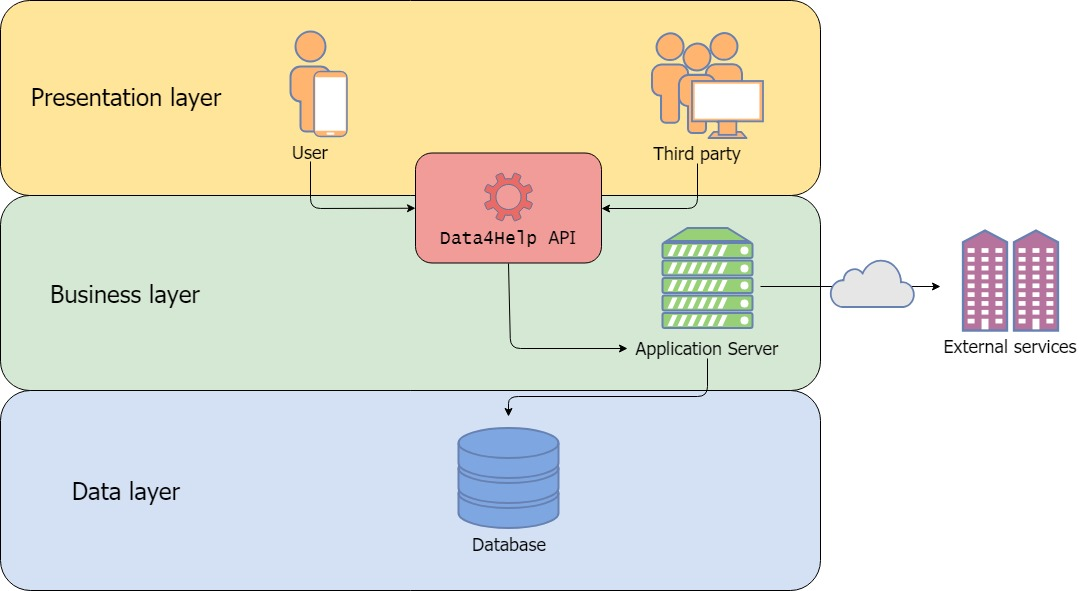
\includegraphics[width=\linewidth]{\fetchImg{util/OverallArchitecture.jpg}}
      \caption{Overall architecture of the system}
      \label{fig:overallarchitecture}
    \end{figure}

    The main components of the system are
    \begin{description}
      \item[App] Application installed on users'devices that communicates with the system; its purpose is to show data to the user and forward his/her requests to the Application Server; we will focus on the smartphone app for Andriod or iOS systems, as it is the main front-end application that our clients need
      \item[Application Server] Back-end component on which the logic of the application takes place; it elaborates the requests it receives and interacts with external services and the data layer; we will focus mainly on this component, as it shall handle all the information dispatching from different layers
      \item[Database] Component responsible for data storage; it shall grant ACID properties (Atomicity, Consistency, Isolation and Durability) and shall provide a management service that handles query parallelization and optimization, as data access policies from different accounts
      \item[External Systems] Systems that interact with \texttt{Data4Help} or \texttt{AutomatedSOS}; they handle functionalities not internally developed in the system, such as payment handling and ambulance dispatching
    \end{description}

  \subsection{Component view}
  \label{sec:compview}

    In this section we will analyze every high-level component in terms of its subcomponents and provide the main interface interaction between different components (Figure~\ref{fig:ComponentDiagram}). For details on component interfaces see Section~\ref{sec:compinterf}.

      \subsubsection{App}

        The application component is the front-end of the system. Our clients will interact with the system through the front end. We will provide
        \begin{itemize}
          \item A smartphone application, capable of exploiting all of the system functionalities: it shall render data, provide forms for the clients (users and third parties) and communicate with the Application Server
          \item An API that allows more experienced users or other developers to automate communication with our system; the API is particularly useful when third parties need to analyze huge quantities of data that a smartphone graphical interface cannot render
        \end{itemize}

        It is important to note that the smartphone application exploits the API for communication with the Application Server. Every \texttt{Data4Help} or \texttt{AutomatedSOS} service can be required by API communication.

      \subsubsection{Application Server}
      \label{sec:applserverinterf}

        The Application Server holds the application logic. It is the only component of the \textit{business} layer, but it is the most crucial component of the system. Its role is to coordinate the information flow between the user layer and the data layer and to incorporate external systems'services.

        In the architecture the Application Server is the only link to the database. External systems or clients cannot directly access persistent data of our system.

        The Application Server is also the only link to the \textit{presentation} layer, as the Application Server  coordinates the user-external system interation.

        Subcomponents of the Application Server are
        \begin{description}
          \item[\AccountManager] This module handles creation, authentication and management of users and third parties'accounts; before exploiting our system's functionalities users and third parties need to be authenticated by this module after providing their credentials
          %check whether the data inserted in the registration phase are correct or not
          % FABIO implicit in "handles creation"
          \item[\DataCollector] This module communicates with users'application and periodically receives data entries, as soon as they're collected by users'wearables
          %user and third party application not only user
          % FABIO only users collect data from wearables, not third parties
          \item[\EmergencyDetector] This module is in charge of automatically analyze data entries inserted in the system if their owner subscribed to \texttt{AutomatedSOS}; it is separated from the \DataCollector\ because emergency detection can be exploited in many ways, depending on the medical literature on the topic; this feature should be independant and isolated from the rest of the architecture
          \item[\EmergencyDispatcher] This module builds emergency messages and forwards them to the SOS system
          \item[\FilterManager] This module composes filter constraints on data entries that can be fetched from the database
          \item[\PaymentGateway] This module is in charge of communicating with the external payment system is order to process payments between third parties and TrackMe
          \item[\RequestManager] This module is in charge of composing, verifying and elaborating third parties'requests, both of single user type and anonymous group type
          \item[\SetBuilder] This module generates data set oriented queries for the database; queries can be accepted or declined by the database, depending on the account permissions concerning data entries access
        \end{description}

      \subsubsection{Database}

        The database is the only component of the \textit{data} layer. Queries are managed by a DBMS that optimizes and elaborates them in parallel. Data stored in the database is persistent and shall not be lost due to external factors. The database service will not be directly developed by us, but will be bought from the existing ones. In Figure~\ref{fig:er} we reported the Entity-Relashionsip diagram for the data stored in the databse.

        The \textit{data} layer is only accessible from the Application Server. It won't implement any application logic, except from DBMS functionalities: it will just respond to queries and passively store data.

        An important factor for \texttt{Data4Help} is the data access policy: Data Entries should be available only to the users that produced them, when inserted in the database. If a Data Set is shared to a third party, that third party shall be allowed to retrive Data Entries that belong to that Data Set from the database. Therefore the access policy shall be dinamic and shall consider \texttt{Data4Help} different accounts.

        \begin{figure}[h!]
          \centering
          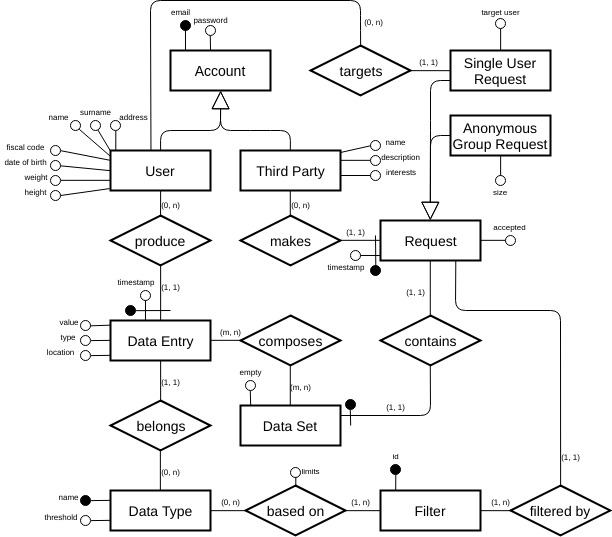
\includegraphics[width=\linewidth]{\fetchImg{util/ER.jpg}}
          \caption{Entity-Relationship diagram for the database}
          \label{fig:er}
        \end{figure}

      \subsubsection{External Systems}

        In this section we will present the main external systems that interact with the Application Server.

        \texttt{Data4Help} relies on an external payment handler. The Application Server, once has composed a third party request, evaluates its price and asks third party for payment, by exploiting the external payment handler service. The service manages the effective payment from the third party to TrackMe and signals errors occurred during the procedure.

        \texttt{AutomatedSOS} relies on an external SOS system. The SOS system dispatches ambulances and handles health emergencies by accepting automated calls. \texttt{AutomatedSOS}, on the Application Server, detects health dangers as soon as they're collected from the front-end components forwards an emergency message to the SOS system.

        \fetchUML
          {ComponentDiagram}
          {UML component diagram of \texttt{Data4Help} and \texttt{AutomatedSOS}: component interaction is described in Section~\ref{sec:deplview} and interfaces are described in Section~\ref{sec:compinterf} and Section~\ref{sec:otherinterfaces}}
          {1}           % scale
          {0}           % move left

  \clearpage
  \subsection{Deployment view}
  \label{sec:deplview}

    % TODO add deployment description
    % TODO add deployment diagram

  \clearpage
  \subsection{Runtime view}
  \label{sec:runtview}

    In this section we will present some sequence diagrams that show the major interaction processes between the system components. All the methods performed between components are described in detail in Section~\ref{sec:compinterf} and Section~\ref{sec:otherinterfaces}.

    %notes (don't delete)
    %orange:user application
    %blue:application server
    %green:database		DBMS		(interact with appserver only)
    %purple:external services		NO :	(interact with appserver only)

    \subsubsection{Account Registration}
    \label{sec:runregistration}

      The sequence diagram in Figure~\ref{fig:run_Registration} shows the registration process to the \texttt{Data4Help} system from the point of view of an user. The same process applies for third parties, by substituting the \texttt{createUserAccount} method with \texttt{createThirdPartyAccount}.

      \fetchUML
        {run_Registration}
        {Account registration to \texttt{Data4Help} system}
        {.7}           % scale
        {0}           % move left

    \clearpage
    \subsubsection{Data entry acquisition}
    \label{sec:userdata}

      The sequence diagram in Figure~\ref{fig:run_AcquireData} shows the process of acquiring a new data entry for a user account, without exploiting \texttt{AutomatedSOS} service. It shows also the login procedure, that is valid for both users and third parties. This procedure will be omitted in the next sequence diagrams, but it shall be performed correctly by every Application involved in the shown processes, in order to be able to exploit all the system functionalities.

      \fetchUML
        {run_AcquireData}
        {Data entry acquisition loop}
        {1}           % scale
        {0}           % move left

    \clearpage
    \subsubsection{Filtering}
    \label{sec:filtering}

      Figure~\ref{fig:run_Filtering} shows the update of graphical data rendering options (see Figure 3 in Section 3.1.1 of the RASD document).

      \fetchUML
        {run_Filtering}
        {Graphical filters selection}
        {1}           % scale
        {0}           % move left

    \clearpage
    \subsubsection{Emergency call}
    \label{sec:automatedSOS}

      In Figure \ref{fig:run_EmergencyCall} we see the \texttt{AutomatedSOS} activation for a user account that was not already subscribed to it and the SOS calling process.

      \fetchUML
        {run_EmergencyCall}
        {Trigger of \texttt{AutomatedSOS} emercency call}
        {1}           % scale
        {0}           % move left

    \clearpage
    \subsubsection{Single User request}
    \label{sec:singleuser}

      The sequence diagram in Figure~\ref{fig:run_SingleUserRequest} shows a third party that performs a single user request. Although it will depend on future TrackMe policies, we added the payment operation to this process.

      \fetchUML
        {run_SingleUserRequest}
        {Single user request elaboration process}
        {1}           % scale
        {0}           % move left

    \clearpage
    \subsubsection{Anonymous Group request}
    \label{sec:anonymousgroup}

      The sequence diagram in Figure~\ref{fig:run_AnonymousGroupRequest} shows a third party that performs an anonymous group request.

      \fetchUML
        {run_AnonymousGroupRequest}
        {Anonymous group request elaboration process}
        {.93}           % scale
        {0}           % move left

    \clearpage

    \subsubsection{Update Single Data}
    \label{sec:updatesingledata}

      The sequence diagram in Figure~\ref{fig:run_SingleUpdate} shows an update process of a given single-user request.

      \fetchUML
        {run_SingleUpdate}
        {Update elaboration process}
        {.93}           % scale
        {0}           % move left

  \clearpage

  \subsubsection{Update Group Data}
    \label{sec:updatedata}

      The sequence diagram in Figure~\ref{fig:run_GroupUpdate} shows an update process of a given anonymous group request.

      \fetchUML
        {run_GroupUpdate}
        {Update elaboration process}
        {.93}           % scale
        {0}           % move left

  \clearpage

  \subsection{Application Server interfaces}
  \label{sec:compinterf}

    In this section we will present the details concerning the interfaces of the subcomponents of Application Server defined in Section~\ref{sec:applserverinterf}. Every component will offer or require some functionalities through interface methods in a way that, once all components are assembled, the Application Server shall not have uncovered functionalities that will not be covered by other systems (Section~\ref{sec:otherinterfaces}). All of this methods has been called at least once in the sequence diagrams of Section~\ref{sec:runtview}.

    \subsubsection{\AccountManager}

      \begin{description}
        \item[\texttt{createUserAccount}] Generates a new user account, provided email, password and other valid information, specified in Section 2.2.1 of RASD document; the return value specifies if the procedure ended correctly or if some incorrect information made it abort
        \item[\texttt{createThirdPartyAccount}] Generates a new third party account, provided email, password and other valid information, specified in Section 2.2.1 of RASD document; the return value specifies if the procedure ended correctly or if some incorrect information made it abort
        \item[\texttt{login}] By providing email and password, a client can login into his/her account and exploit system functionalities\footnote{the \textit{login} procedure is exploited, according to the stateless communication paradigm, by providing the credentials to every request from the client side, in order to guarantee isolation between the requests}; the return value is positive if information provided is correct and negative if there's no account that matches given credentials
        %\item[\texttt{resetPassword}] This method is called when a client doesn't remember his/her password: it triggers a reset procedure through the client's email, used for registering to \texttt{Data4Help}
        \item[\texttt{editInfo}] Updates the client's profile information with the the new set of information passed as parameter; the return value confirms if the procedure ended correctly; it may even toggle \texttt{AutomatedSOS} real time health danger detenction checks on inserted data
        %\item[\texttt{toggleAutomatedSOS}] Activates or stops \texttt{AutomatedSOS} health danger real time checks on inserted data entries in the system
        %\item[\texttt{getSharingPermissions}] This method returns the set of data types that the target user is willing to share anonymously
      \end{description}

    \subsubsection{\DataCollector}
    \label{sec:datacollectormethod}
      \begin{description}
        \item[\texttt{acquireNewDataEntry}] This method acquires a new data entry collected on the logged user's application; if the logged user is subscribed to \texttt{AutomatedSOS}, it forwards the data entry to the \EmergencyDetector
      \end{description}

    \subsubsection{\EmergencyDetector}

      \begin{description}
        \item[\texttt{analyzeDataEntry}] This method analyzes passed data entry and checks whether all parameters are above or below defined thresholds; if some parameters exceed thresholds, it will call the \EmergencyDispatcher\ in order to forward the SOS call
        %\item[\texttt{generateEmergencyMessage}] This method, given a data entry that exceedes thresholds, returns an emergency message that must be delivered to the SOS system
      \end{description}

    \subsubsection{\EmergencyDispatcher}

      \begin{description}
        \item[\texttt{sendEmergencyMessage}] This method builds and forwards an emergency message to the SOS system
      \end{description}

    \subsubsection{\FilterManager}

      \begin{description}
        \item[\texttt{generateFilter}] This method returns a new filter instance with the passed parameters on type and boundaries of data, that can be used to narrow the data domain of interrogation during database queries; the return value specifies if the filter is well formed or if it cannot be created
      \end{description}

    \subsubsection{\PaymentGateway}

      \begin{description}
        \item[\texttt{pay}] This method triggers a payment call to the external payment system that returns a positive or negative exit status, depending on the correct execution of the procedure; the return value contains the errors of the payment procedures
      \end{description}

    \subsubsection{\RequestManager}

      \begin{description}
        \item[\texttt{makeSingleUserRequest}] This method, provided a target user and the proper filters over the data that the third party wants to collect, generates a new single user request by the third party for the target user's data; it returns the data set that contains the requested data if the procedure ended correctly or a notification error, if the user declined the request
        \item[\texttt{makeAnonymousGroupRequest}] This method, provided the proper filters over the data that the third party wants to collect, generates a new anonymous group request; it returns the data set that contains the requested data if the procedure ended correctly or a notification error, if the system wasn't able to properly anonymize the data set
        \item[\texttt{updateData}]  This method, provided that a single-user or anonymous-group request has been previously done by the third party; it returns either the new user-data stored in the database since the last update(not already shared with the third party) or an error message if the user, meantime, has revoke the consensus for that single-user request
      \end{description}

    \subsubsection{\SetBuilder}

      \begin{description}
        \item[\texttt{getDataSet}] This method accepts some filters as parameters and forwards a query based on such filters to the database (filters shall be previously elaborated by \FilterManager); the return value is either the set of data entries fetched from the database subject to the filter's constraints or an error message if the \FilterManager request couldn't be performed (the asking user hasn't access permissions or in the database there aren't enough data to satisfy the query requirements)
      \end{description}

  \subsection{Other interfaces}
  \label{sec:otherinterfaces}

    In this section we will explore the interface methods of the components that communicate with the Application Server. These components rely on external services and their interfaces may be very complex and may change over time, due to the fact that in the most cases, we are not directly developing them. Therefore our description is at a high level of abstraction. Furthermore, we will focus only on the critical methods that are mandatory for the system in order to communicate correctly with the Application Server.

    \subsubsection{Application}

      The following methods are not called by the Application Server, but are useful in order to understand the expected behaviour of the Application when recieving data from the Application Server.

      \begin{description}
        \item[\texttt{renderDataSet}] Visually renders a data set on the application screen
        \item[\texttt{showNotification}] Shows a notification error or a data request notification (in case of user account targeted by a third party single user request) on the application screen
      \end{description}

    \subsubsection{Database}

      \begin{description}
        \item[\texttt{addAccount}] This method adds a new user or third party account to the account set of the system; the return value states if the procedure ended correctly
        \item[\texttt{requstData}] This method analyzes the passed query throug the DBMS service in parallel with other queries and returns the tuples corresponding to the required data, or returns an error if the asking account hasn't the permissions to read the data
        \item[\texttt{saveData}] This method saves the passed data into the persistent memory
        \item[\texttt{updatePermissions}] This method updates permission accesses to data entries of the system, in order to share them between user and third party accounts; the return value states the correct ending of the procedure
      \end{description}

    \subsubsection{External Systems}

      Payment system and SOS system are the only external systems required by the Application Server. The payment system offers
      \begin{description}
        \item[\texttt{processPayment}] This method accepts payment data and performs the effetive money movement from third party to TrackMe; it returns the exit status of the process, positive if it ended correctly or negative, alongside an error log, if the process was not succesfull
      \end{description}
      while the SOS system offers
      \begin{description}
        \item[\texttt{sendEmergency}] This method accepts emergency messages and dispatches ambulances according to the data contained in the passed emergency message
      \end{description}

  \subsection{Selected architectural sytles and patterns}
  \label{sec:stylesandpatterns}

    \begin{description}
      \item[Model-View-Controller] We adopted the MVC pattern because it separates the three most important architectural aspects of the system: data storage, user interfaces and business logic. It allows to develop in parrallel every component, in isolation from the others, granting a less error prone developement and a more extensible architecture to future additions or punctual changes. The MVC pattern can be adopted at varoius architectural levels, as we can find it also in the mobile application.

      \item[Three-tier architecture] It allows to develop in isolation the presentation layer, the business layer and the data layer. It allows also to deploy on different physical nodes these layers, enhancing the MVC paradigm and the complete isolation of the layer components. The physical separation of nodes enhances reliability and availability of the services, as the application logic and data may be distributed on more than one node, lowering the failure probability and enhancing overall performances.
      \item[Client-Server] It is the standard model of communication of the World Wide Web.

      \item[Thin client] Data and logic of the system are handled in the data and business layer respectively. The presentation layer has the only role of showing data to the user and performing requests that will be handled by the other layers. (Figure~\ref{fig:thinclient}). In this way \texttt{Maintanability} and \texttt{Availability} are granted despite software and hardware updates of smartphones.

      \item[REST and stateless communication] In order to make the system scalable with the number of requests, it is a good practice to grant stateless communication between client and server. According to the REST paradigm, every HTTP request encapsulates all the data needed to be performed, therefore it is completely independant from other requests. This paradigm allows different requests to be handled from different server nodes, encreasing scalability possibilities and load balancing options. The server doesn't hold any session information about the client.
    \end{description}

    \begin{figure}[h!]
      \centering
      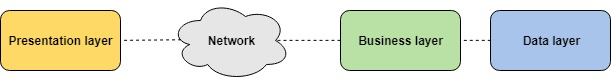
\includegraphics[width=.85\linewidth]{\fetchImg{util/ThinClient.jpg}}
      \caption{Thin client architecture: logic operations and data storage are not performed by the client nodes, on which the presentation layer reside}
      \label{fig:thinclient}
    \end{figure}

  \subsection{Other design decisions}
  \label{sec:designdecisions}
  Data collection is a very critical functionality for both AutomatedSOS and Data4Help.
  Despite the fact that are two separate elements, deciding to have two different data collection subcomponents in ~\ref{sec:applserverinterf} will result in a significant drawback:the reduction of \texttt{Maintanability} which, as already said in section 3.7.4 of the RASD document, is a very important aspect of our software.
  This is the reason why in ~\ref{sec:datacollectormethod} is said that \EmergencyDetector  retrieve user's health parameters from \DataCollector  and not collects them directly to the app: in this way any change in the physical wearables deviced will requires the update only of \DataCollector  while \EmergencyDetector  remains the same; thus the software Manintanability is increased.  


\end{document}
